\documentclass[a4paper,12pt]{article}
\usepackage{graphicx}
\usepackage{fancyhdr}
\usepackage{xcolor}
\usepackage[table]{xcolor}
\usepackage{hyperref}
\usepackage{booktabs}
\usepackage{indentfirst}
\usepackage{subcaption}

\setlength{\arrayrulewidth}{0.5mm}
\setlength{\tabcolsep}{18pt}
\renewcommand{\arraystretch}{2.5}

\pagestyle{fancy}

\fancyhf{} 
\fancyfoot[L]{\textcolor{teal}{\rule[0mm]{0.45\linewidth}{2pt}}} 
\fancyfoot[R]{\textcolor{teal}{\rule[0mm]{0.45\linewidth}{2pt}}} 

\fancyfoot[C]{\thepage}

\renewcommand{\contentsname}{\textcolor{teal}{Table of Contents}}

\begin{document}

\begin{titlepage}
    \begin{center}
        \vspace*{2cm}

        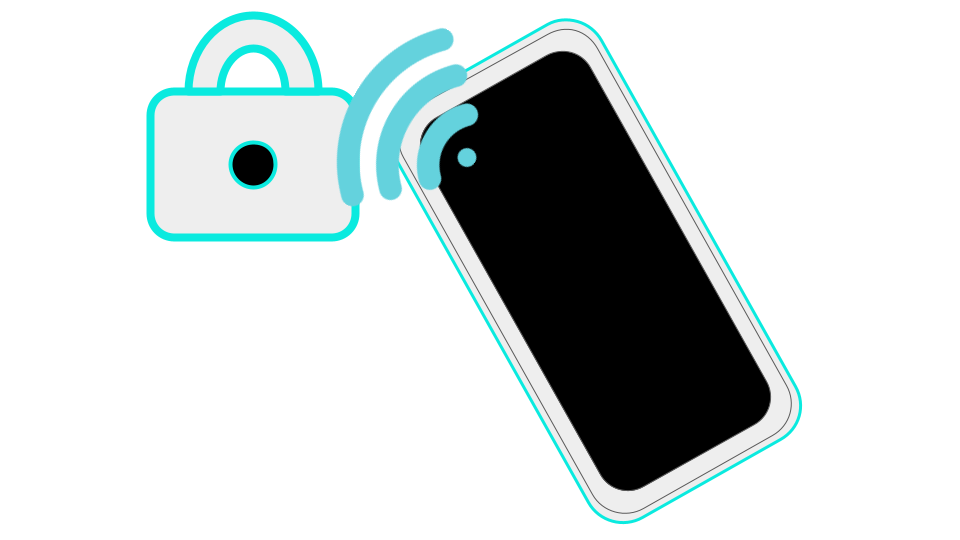
\includegraphics[width=0.8\textwidth]{./img/slimg.png}\\[1cm]

        {\Huge \textbf{Smart Lock}}\\[0.5cm]
        {\textcolor{teal}{\Large A Cloud-Based Key}}\\[1.5cm]

        {\LARGE \textbf{Group 5}}\\[0.5cm]
        {\Large \textit{Nathaniel Laurente, Adam Wu, Neena Nguyen, Jackson Kennedy}}\\[2cm]

        {\Large \today}
    \end{center}
\end{titlepage}

\newpage
\pagenumbering{arabic}
\pagestyle{fancy}      



% BEGIN DOCUMENT -------------------------------------------------------------------------


\section{Front Matter}

% Executive Summary
\section*{\textcolor{gray}{Executive Summary}}

In an era where security and convenience are necessary, traditional lock-and-key systems are becoming outdated. Lost keys, forgotten access codes, and lack of remote control present serious challenges for homeowners and businesses alike. Our Auto Smart Lock project is a solution designed to enhance security while offering friendly user accessibility.
\newline
Our goal is to develop a smart lock that integrates modern authentication methods with remote access capabilities. By leveraging an ESP32-C3 microcontroller in conjunction with Firebase cloud services, our smart lock enables users to lock and unlock their doors from anywhere, eliminating the risks associated with traditional keys.
\newline

At the core of our smart lock is an ESP32-C3 microcontroller, which connects to WiFi and Firebase cloud services to securely manage lock and unlock commands. When a user enters a PIN or sends a command from their phone, the system checks if the code is valid. If it is, the solenoid lock is triggered, unlocking the door. We’ve designed the lock to be fast, secure, and easy to install, with a 3D-printed casing to house the components.
\newline

Before finalizing the prototype, we are running key tests to ensure everything works smoothly. These tests check if the phone properly connects to the lock, if the lock responds quickly, if multiple users can access it without conflicts, and if temporary PINs expire when they should. Our next steps include assembling all parts, optimizing performance, and making sure the system is fully secure and reliable. By the end of Winter 2025, we aim to have a fully functional smart lock prototype that provides a safer, smarter, and more convenient way to secure homes.

% Ethics Statement
\newpage
\section*{\textcolor{gray}{Ethics Statement for Smart Lock Project}}
Our Smart Lock is designed to enhance security and convenience for users while upholding ethical standards in privacy, safety, and accessibility. We recognize our responsibility to develop and deploy technology that prioritizes ethical considerations in the following ways:

\textcolor{teal}{\subsection*{Privacy and Data Protection}}
We are committed to safeguarding user privacy by:
\begin{itemize}
    \item Minimizing data collection to only essential information required for functionality.
    \item Implementing encryption and secure authentication methods to prevent unauthorized access.
    \item Ensuring that user data is never shared or sold to third parties without explicit consent.
\end{itemize}

\textcolor{teal}{\subsection*{Security and Reliability}}
To maintain the integrity of the smart lock system, we will:
\begin{itemize}
    \item Use cybersecurity measures to prevent hacking and tampering.
    \item Regularly update software and firmware to address potential vulnerabilities.
    \item Ensure the lock functions reliably under various conditions to prevent accidental lockouts or failures.
\end{itemize}

\textcolor{teal}{\subsection*{User Safety and Accessibility}}
We aim to create a system that is safe and inclusive by:
\begin{itemize}
    \item Designing intuitive user interfaces for easy access by individuals with different levels of technical proficiency.
    \item Ensuring compliance with accessibility standards for individuals with disabilities.
\end{itemize}

\textcolor{teal}{\subsection*{Ethical Use and Non-Discrimination}}
The smart lock must be used ethically and responsibly by:
\begin{itemize}
    \item Preventing misuse that could lead to unauthorized surveillance or discrimination.
    \item Avoiding biases in authentication methods that may disadvantage certain user demographics.
\end{itemize}

\textcolor{teal}{\subsection*{Transparency and Accountability}}
To uphold ethical standards, we will:
\begin{itemize}
    \item Clearly communicate to users how their data is handled and stored.
    \item Provide documentation on security features, risks, and best practices.
    \item Accept feedback and take responsibility for any ethical concerns that may arise during development and deployment.
\end{itemize}

By adhering to these ethical principles, we ensure that our Smart Lock product aligns with values of privacy, security, fairness, and social responsibility.


\tableofcontents
\newpage

\section{Background}

\subsection*{Persona 1: Marcus Lee}

%%% 
\begin{itemize}
    \item Background: 
    \begin{itemize}
        \item Homeowner, 42 years old, IT Manager, Lives in a suburban neighborhood
    \end{itemize}

    \item Goals:
    \begin{itemize}
        \item Secure keyless entry for family
        \item Enable remote monitoring when traveling
        \item Integrate smart lock with his existing smart home system
    \end{itemize}

    \item Behaviors:
    \begin{itemize}
        \item Uses smart home apps
        \item Values reliability and ease of setup over complex features
    \end{itemize}

    \item Traits:
    \begin{itemize}
        \item Security-conscious
        \item Tech-savvy
        \item Efficiency-driven
    \end{itemize}
\end{itemize}

% \begin{figure}[!ht]
%     \centering
%     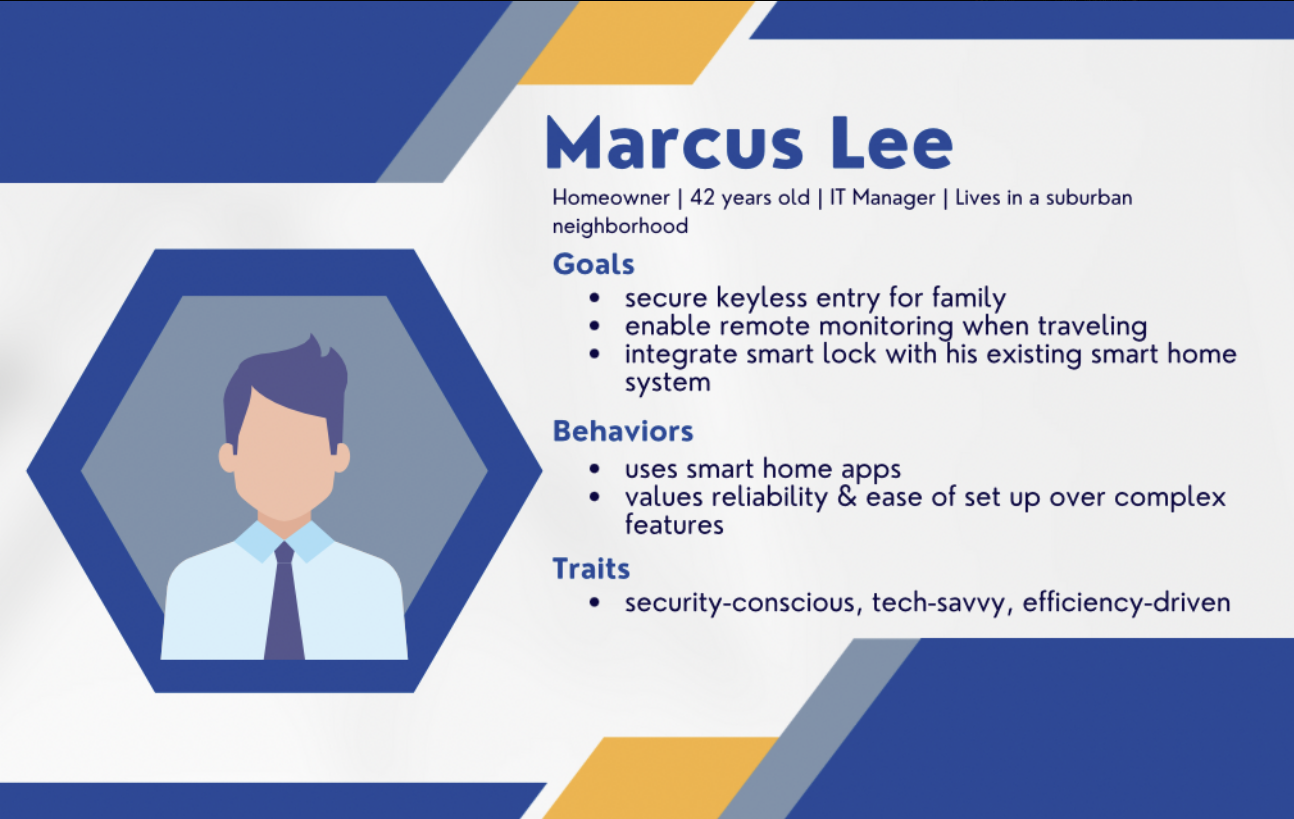
\includegraphics[width=110mm,scale=0.4]{./img/Persona1.png}
%     \label{fig:persona1}
% \end{figure}

\subsection*{Persona 2}
\begin{figure}[!ht]
    \centering
    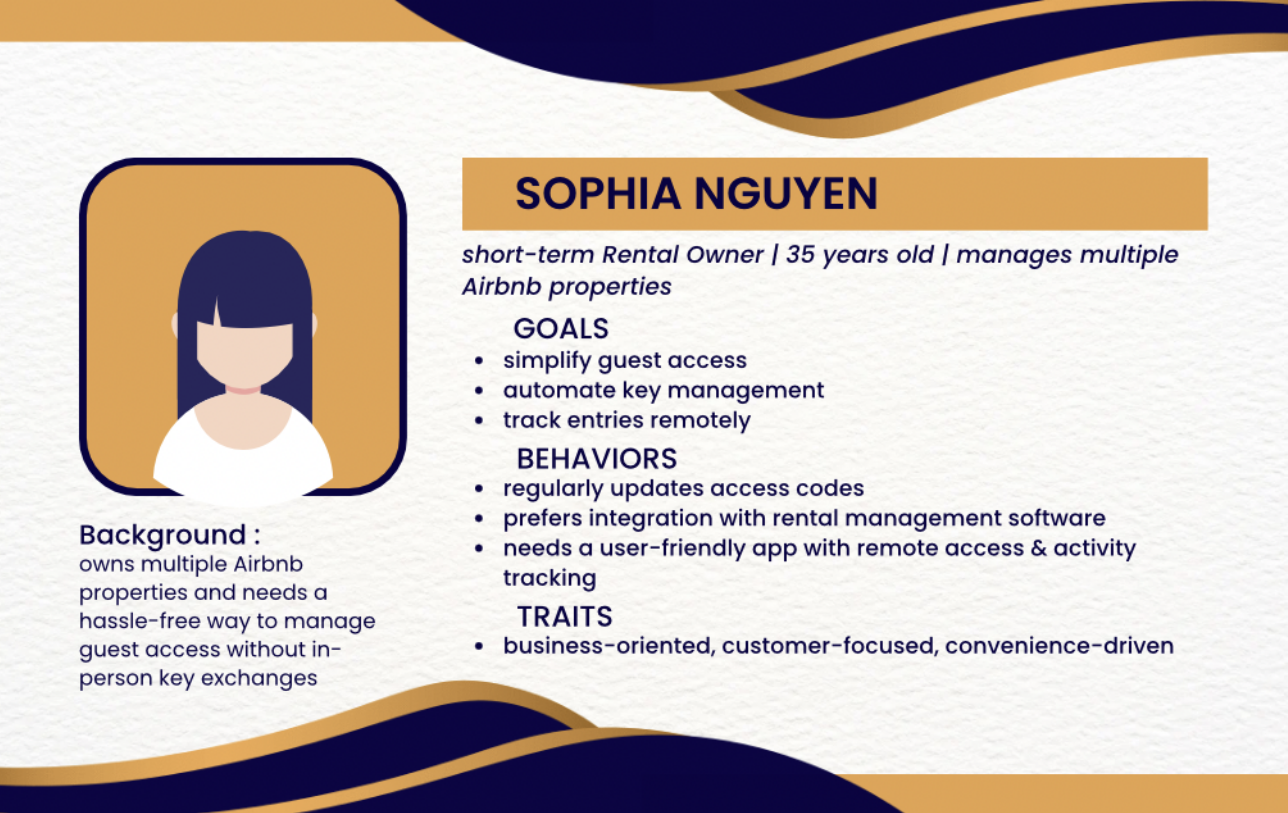
\includegraphics[width=110mm,scale=0.4]{./img/Persona2.png}
    \label{fig:persona2}
\end{figure}
\newpage



\subsection{Problem Definition}

\subsubsection{Need \& Goal Statements}
\begin{itemize}
    \item Need Statement - Traditional lock-and-key systems are inconvenient and insecure, as users may forget, lose, or have their keys stolen. Additionally, they obviously lack remote access, making it difficult for someone to enter the building if someone lost/forgot their tiny key.
    
    \item Goal Statement - Our smart lock will address these issues by enabling remote locking and unlocking, getting rid of the need for physical keys, and ensuring secure authentication for authorized users.
\end{itemize}


\subsubsection{Design Objectives}
\begin{itemize}
    \item Remote access \& control: ESP32-C3 connection with Firebase
    
    \item Local authentication via keypad:
    \item Store \& validate PINs securely using Firebase cloud
    \item Multi-user support
    \item solenoid lock integration with ESP32

\end{itemize}

\newpage
\section{Concepts Considered}

\subsection{6-3-5 Method}
\subsubsection*{Hardware \& Mechanics}
\begin{itemize}
    \item use a servo motor for deadbolt control
    \item hall effect sensor to detect if the door is open or closed
    \item implement linear actuator for silent locking
    \item maybe anti-backlash gears to reduce mechanical play
    \item consider designing a modular lock housing with 3D-printed parts
    \item have a backup battery to ensure operation during power outages
\end{itemize}

\subsubsection*{Smartphone Integration}
\begin{itemize}
    \item develop a smartphone app for remote locking/unlocking
    \item push notifications for lock activity (ex: ``Door locked at 3:45 PM'')
    \item have biometric authentication (Face ID or fingerprint)
    \item Use Bluetooth for proximity-based auto-unlock
    \item NFC support for quick unlocking via phone tap
    \item include multi-user access control with time-based permissions
\end{itemize}

\subsubsection*{Security Features}
\begin{itemize}
    \item Implement AES-256 encryption for communication between the lock and phone
    \item maybe two-factor authentication for app access
    \item develop a tamper-detection alarm if the lock is forced
    \item lockdown mode for multiple failed attempts
    \item include a manual override mechanism in case of system failure
    \item utilize rolling codes for Bluetooth pairing to prevent hacking
\end{itemize}

\subsubsection*{Software \& Control}
\begin{itemize}
    \item ESP32 microcontroller for Wi-Fi and Bluetooth control
    \item Develop a closed-loop system to verify if the lock is engaged properly
    \item make a real-time event log accessible via the app
    \item add a scheduling feature for auto-locking at specific times
    \item guest mode with temporary passcodes
    \item Integration with voice assistants like Alexa or Google Assistant
\end{itemize}

\subsubsection*{Advanced Features}
\begin{itemize}
    \item GPS stuff
    \item add geofencing to lock or unlock based on the user's location
    \item integrate with smart home platforms like Home Assistant
    \item use AI-based behavior analysis to suggest locking patterns
    \item add a camera with facial recognition for auto-unlock
    \item enable remote firmware updates
    \item learn database SQL
    \item use solar charging for battery-powered locks
\end{itemize}



% BRAINSTORMING -----------------------------




\subsection{Brainstorming}

\subsubsection*{Adam Wu}
\begin{itemize}
    \item As a person who has amnesia, I would like to be able to find my keys anytime so that when I forget where I place them, I can find them.
    \begin{itemize}
        \item Having a "find my" solution with a key.
    \end{itemize}
    \item As a person who loves security, I would like to have the best lock for my house so that lock pickers are not able to pick my lock.
    \begin{itemize}
        \item Making an “authentication” key that resets the key code within a set time, making it harder for hackers to unlock the door.
    \end{itemize}
    \item As a person who is always last-minute out the door, I fear forgetting to lock the door when I close it.
    \begin{itemize}
        \item Auto-locking door when a person closes the door.
    \end{itemize}
    \item As a person who often forgets to bring their keys, I am scared of getting locked out.
    \begin{itemize}
        \item Having a notification from the key to the phone that alerts: “keys are not close by to you.”
    \end{itemize}
    \item As a parent, I am scared of my kids forgetting their keys and locking themselves out of their room.
    \begin{itemize}
        \item Creating a “master key” that only parents/admins can use to unlock specific doors.
    \end{itemize}
    \item Concerned about key battery life.
    \begin{itemize}
        \item Send a notification to the user when the key is on low battery.
    \end{itemize}
\end{itemize}

\subsubsection*{Nathaniel Laurente}
\begin{itemize}
    \item Key has the ability to notify the user when too far away from the user’s phone/body.
    \item Key deactivates/won’t be able to open the door if too far away from the owner.
    \item “Tap to Pay” technology concept.
    \begin{itemize}
        \item Unlocks the door like a credit card tap on a phone.
        \item If too complex, explore alternative ways to unlock the door.
        \item Eliminates the need for a physical key.
        \item Prevents stolen keys from working if the user still has their phone.
    \end{itemize}
    \item Secure deactivation of the key when too far from the user.
    \begin{itemize}
        \item Possible solution: Use the user's phone for deactivation.
    \end{itemize}
    \item One-time password generator between lock and key to ensure only this exact key can enter the house.
    \item Backup way to get into the house if the user forgets/loses their key.
    \begin{itemize}
        \item Pin access code.
        \item App allows for 2FA authentication using a thumbprint and/or Face ID.
    \end{itemize}
    \item Will the battery last long enough for multiple years?
\end{itemize}

\subsubsection*{Neena Nguyen}
\begin{itemize}
    \item Existing smart lock solutions:
    \begin{itemize}
        \item Smart locks for dorm rooms using mobile apps, passcodes, and scanners.
    \end{itemize}
    \item Who will use this lock?
    \begin{itemize}
        \item People with memory issues (elderly, ADHD).
        \item University students in dorm rooms.
        \item Student ID scanner integration.
        \item Parents with small children (child-proof locks).
    \end{itemize}
    \item Features for parental control.
    \begin{itemize}
        \item Locks after a curfew time.
        \item Prevents children from unlocking without parental approval.
        \item Alerts parents when kids come home from school.
    \end{itemize}
    \item What kind of door lock will it be?
    \begin{itemize}
        \item Facial recognition (requires camera and database knowledge).
        \item Logs entry and exit timestamps.
        \item Digital passcode through an app.
        \item Auto-relocking mechanism after failed attempts.
        \item Bluetooth detection for unlocking within a certain range.
        \item Dual authentication (PIN + scan).
        \item Optional security trigger after specific hours.
        \item Alerts when the door is left unlocked for too long.
        \item Auto-locking after prolonged unlocking.
        \item Detection system to check if the key is on the person.
        \item Prevents intruders from entering without a key.
    \end{itemize}
\end{itemize}

\subsubsection*{Jackson Kennedy}
\begin{itemize}
    \item Normal keys can be lock-picked, but digital keys can be secured based on a communication protocol.
    \item Secure authentication methods.
    \begin{itemize}
        \item PIN authentication with 2FA.
        \item Optimal PIN length (e.g., 4-digit PIN has 1,048,576 combinations).
        \item Brute force prevention strategies.
    \end{itemize}
    \item Preventing communication protocol vulnerabilities.
    \begin{itemize}
        \item What protocol should be used? (Bluetooth has vulnerabilities and short range.)
        \item Cloud-based solutions rely on third-party vendor security.
        \item What information needs to be transferred? (Video data, authentication signals?)
    \end{itemize}
    \item Lock activation logic.
    \begin{itemize}
        \item How exactly will the lock know when to unlock? (Sending a 0 or 1 signal based on specific conditions?)
    \end{itemize}
    \item Security and alerting technologies.
    \begin{itemize}
        \item Sensors to detect nearby people.
        \item Hidden camera or biometric verification for identity confirmation.
    \end{itemize}
    \item Scheduling and timed access.
    \begin{itemize}
        \item Physical locks do not have scheduling options.
        \item Implement timed unlocking (e.g., unlock for 15 minutes for a babysitter).
        \item Extra verification to prevent intruders from exploiting schedules.
    \end{itemize}
\end{itemize}
\newpage









% Begin Morphological Charts ----------------------------------

\subsection{Morphological Charts}

\begin{figure}[!ht]
    \centering
    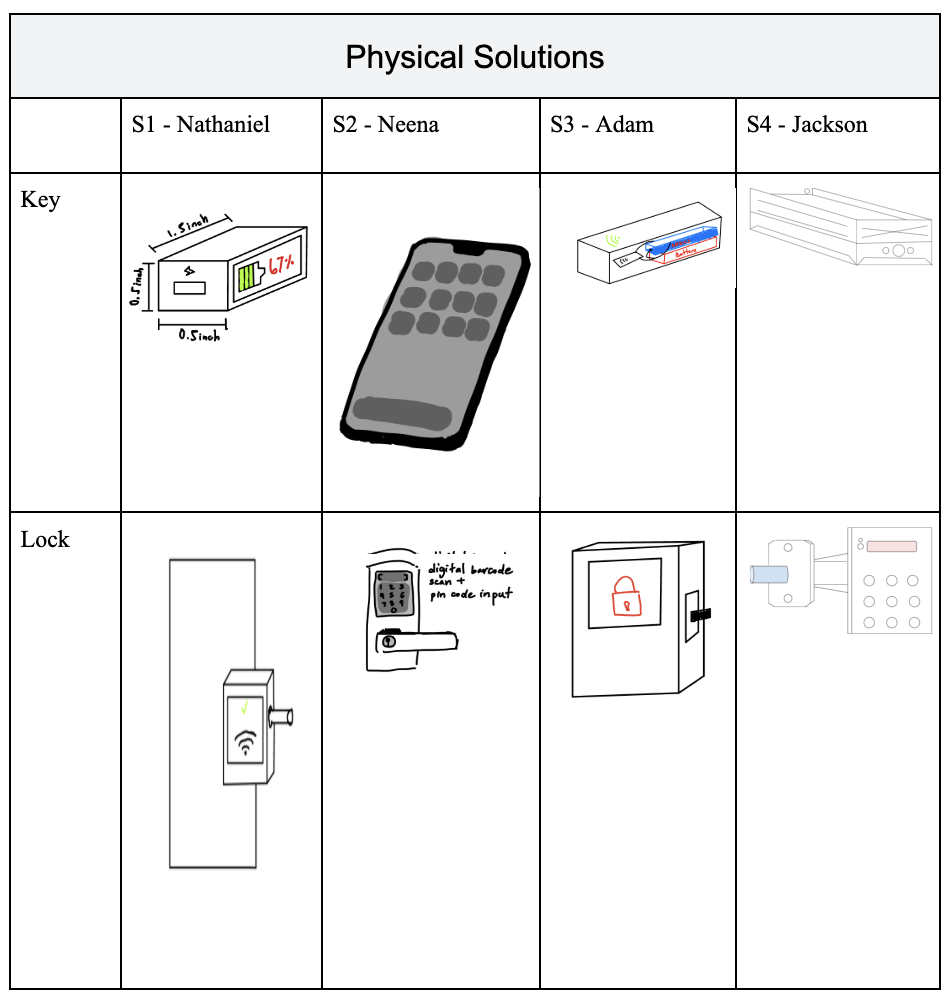
\includegraphics[width=1\linewidth]{./img/p1mm.png}
    \caption{Physical Solution Chart}
    \label{fig:p1mm}
\end{figure}
\newpage
\begin{figure}[!ht]
    \centering
    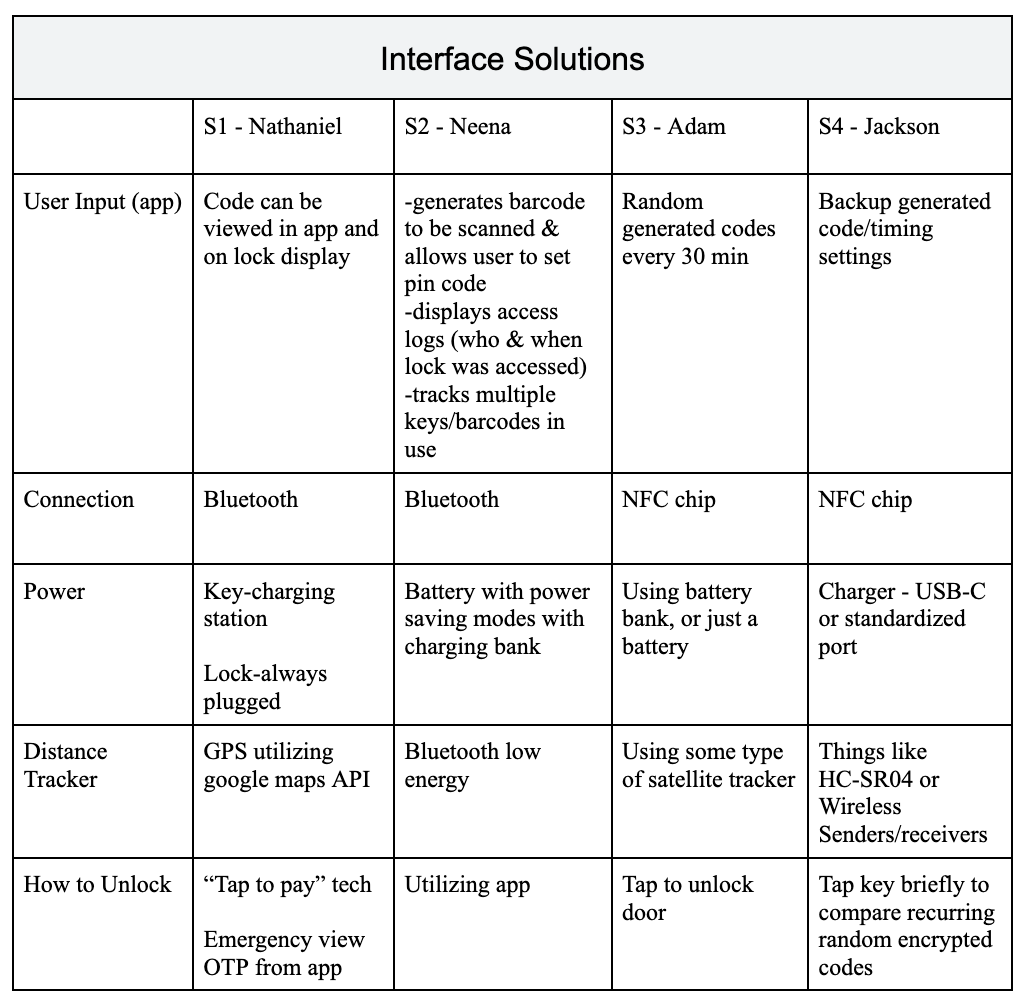
\includegraphics[width=1\linewidth]{./img/p2mm.png}
    \caption{Interface Solutions}
    \label{fig:p2mm}
\end{figure}
\newpage





% Begin Mind Map ---------------------------------------------

\subsection{Mind Map}

\begin{figure}[!ht]
    \centering
    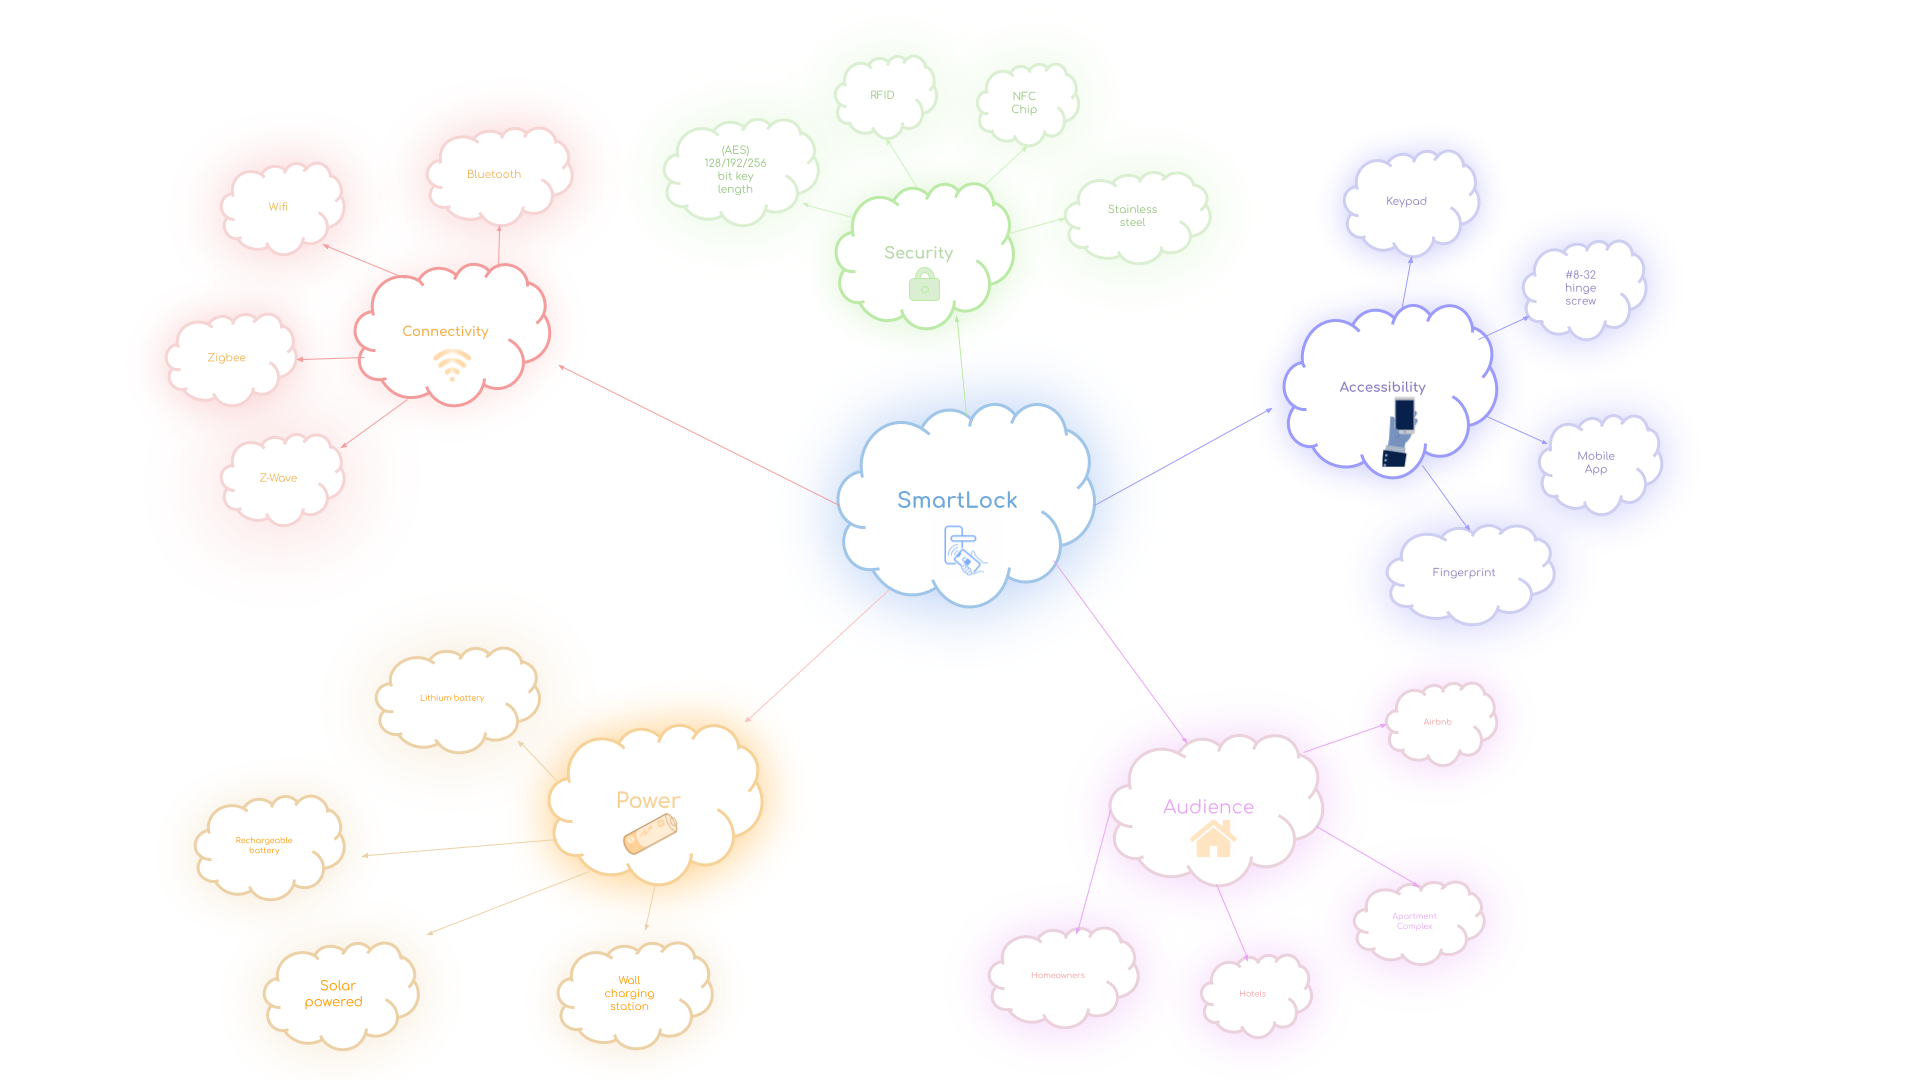
\includegraphics[width=140mm,scale=0.5]{./img/mindmapsmartlock.png}
    \caption{Mind Map}
    \label{fig:mindmapsmartlock}
\end{figure}
\newpage

\subsection{Concept Selection}

\subsubsection{Weighting Factors}
\begin{tabular}{ll}
    \toprule
    Criteria & Weight (\%) \\
    \midrule
    Security & 40 \\
    Cost & 30 \\
    Power Consumption & 20 \\
    User Convenience & 10 \\
    \textbf{Total} & \textbf{100} \\
    \bottomrule
\end{tabular}

\subsubsection{Decision Table}
\resizebox{\textwidth}{!}{%
\begin{tabular}{lcccc}
    \toprule
    Criteria & Weight & Design 1 (Basic) & Design 2 (Mid-Range) & Design 3 (Advanced) \\
    \midrule
    Security & 40 & 6 (240) & 8 (320) & 10 (400) \\
    Cost & 30 & 10 (250) & 6 (150) & 3 (75) \\
    Power Consumption & 20 & 6 (90) & 8 (120) & 10 (150) \\
    User Convenience & 10 & 3 (30) & 6 (60) & 9 (90) \\
    \textbf{Total Score} & \textbf{100} & \textbf{680} & \textbf{720} & \textbf{780} \\
    \bottomrule
\end{tabular}%
}

\textbf{Best Design:} Design 3 (Advanced) with 780 points, prioritizing security, cost-efficiency, and power optimization.

\newpage


% Design of Manufacture addition
\subsection{\textcolor{gray}{Detail of Design}}
The Smart Lock prototype consists of both hardware and software components, designed to provide secure, remote access control with user authentication and cloud connectivity.

\subsubsection{\textcolor{teal}{System Overview}}

Our system integrates a physical keypad-based lock with Wi-Fi-enabled remote access through a mobile application. Users can authenticate using a PIN or biometric authentication (fingerprint or facial recognition), and manage access remotely.

\begin{figure}[h]
    \centering
    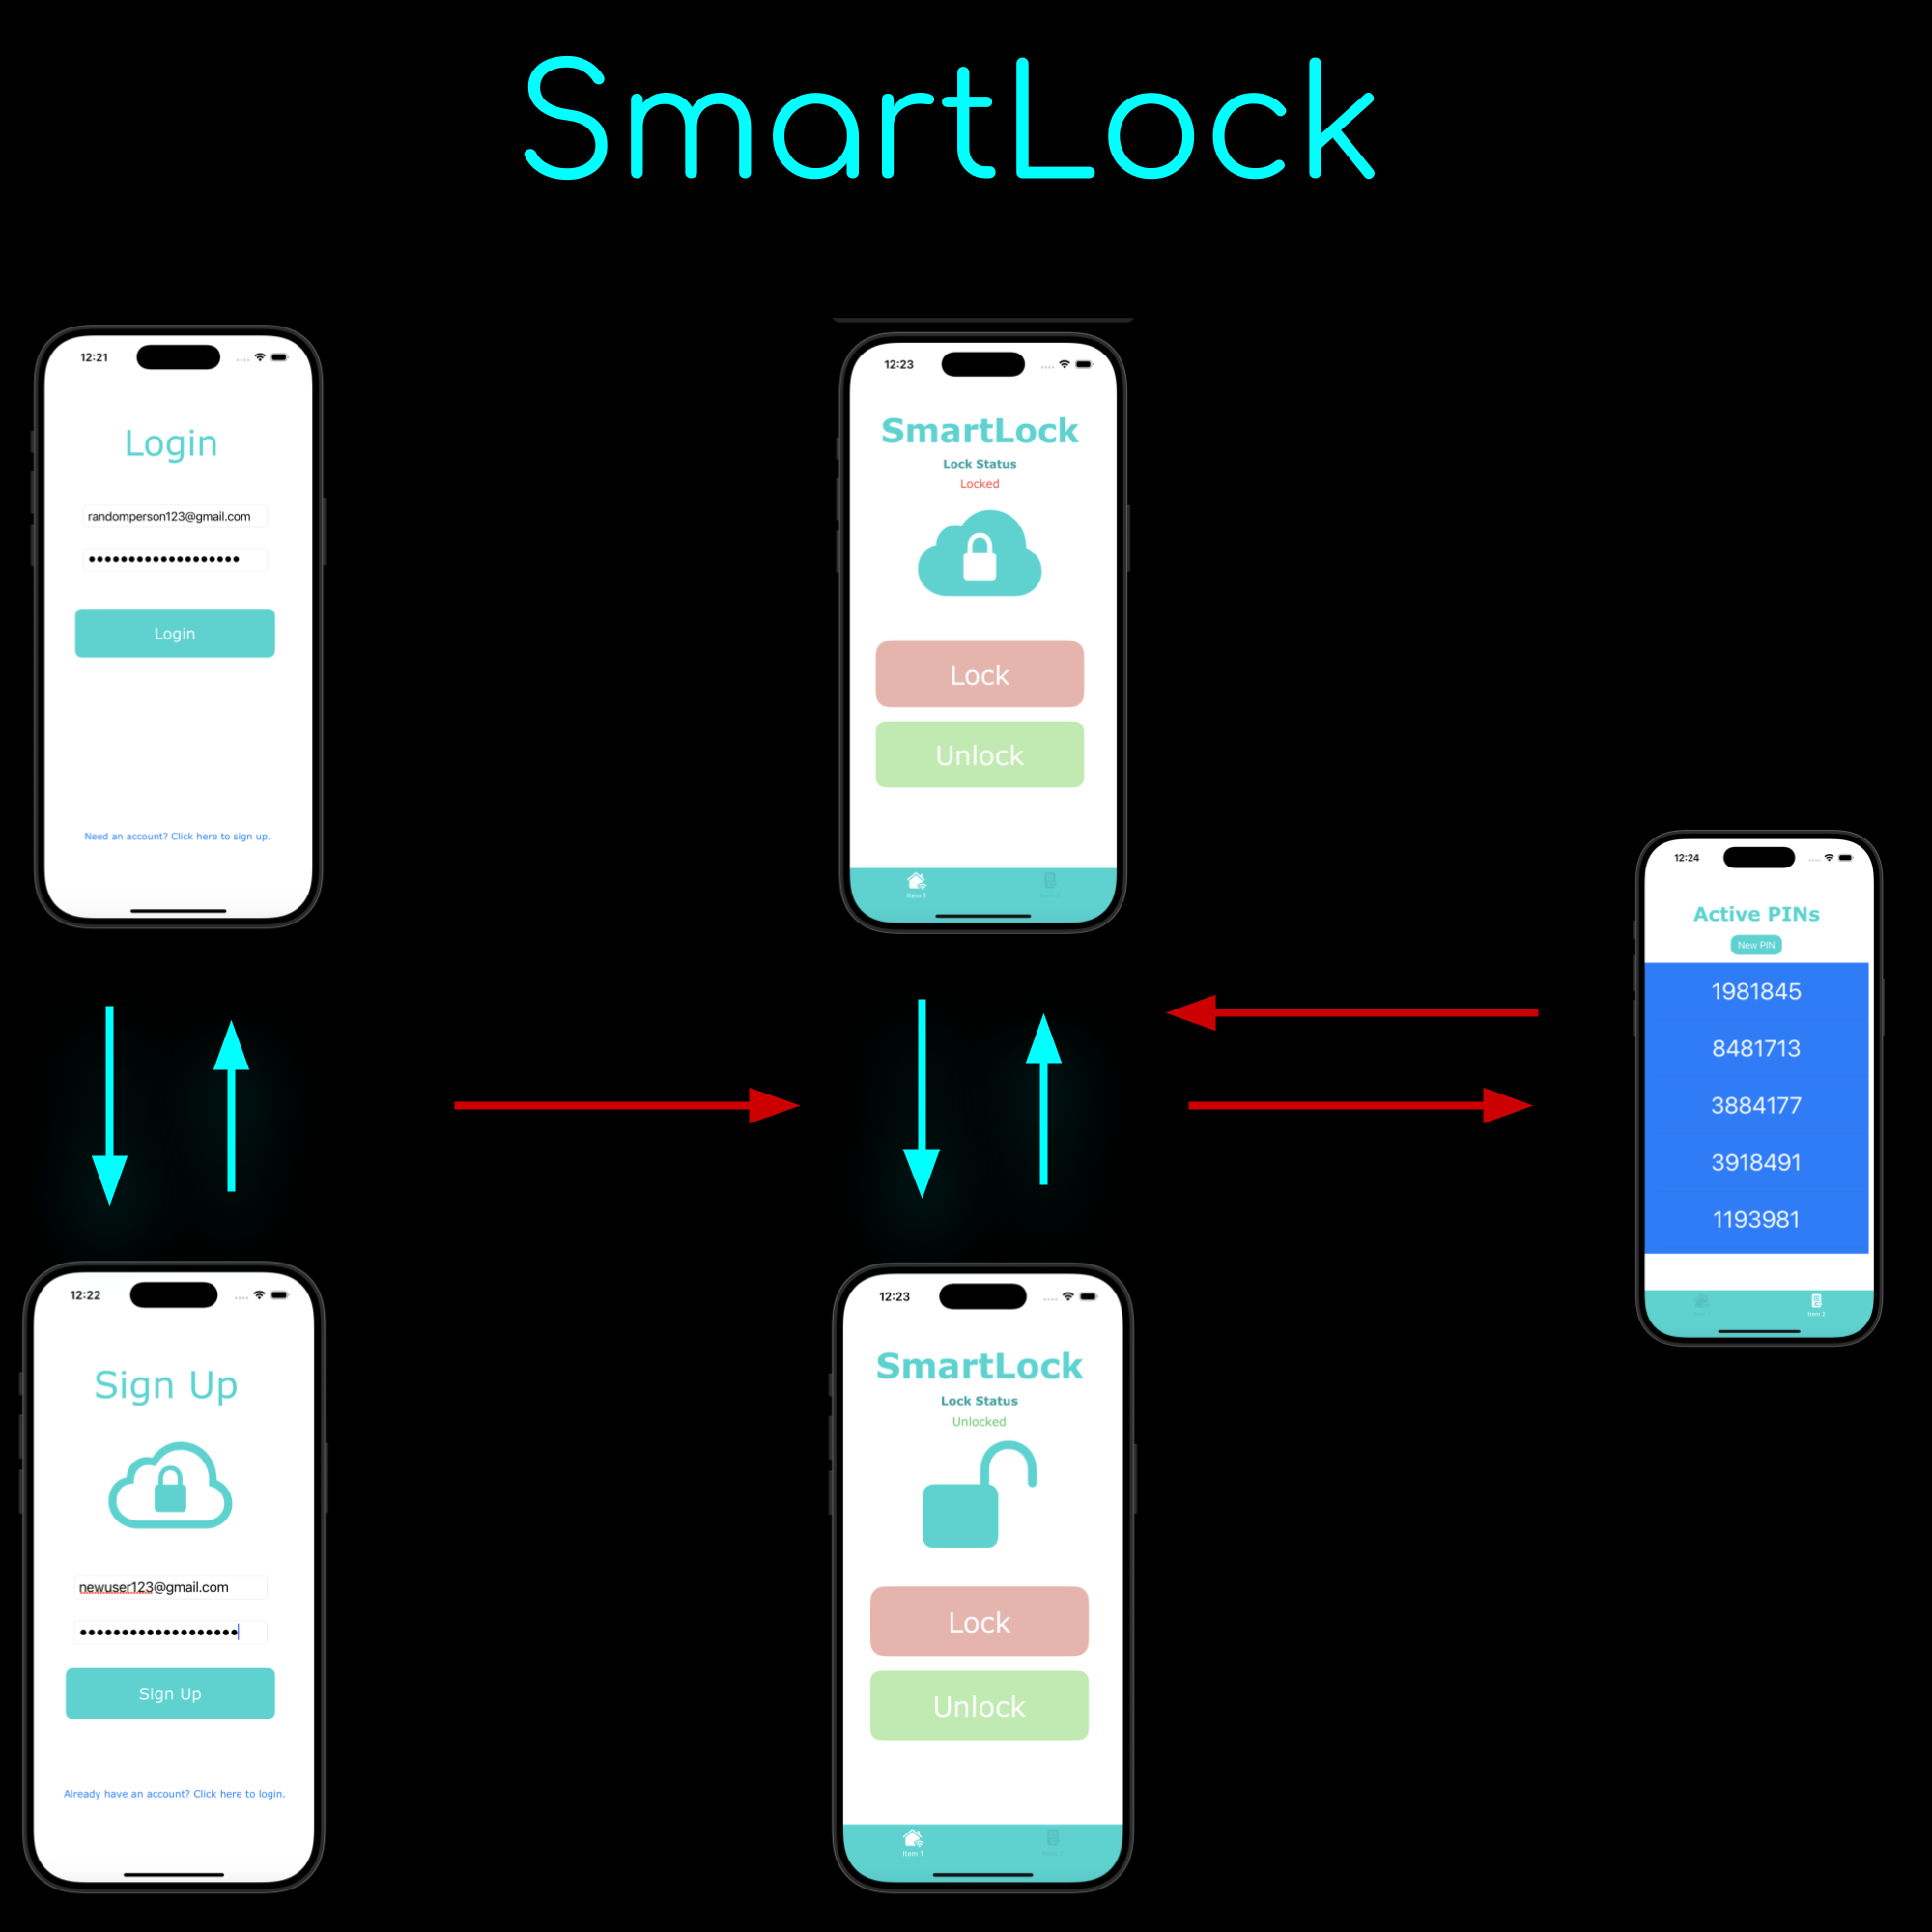
\includegraphics[width=0.65\textwidth]{flowsl.png}
    \caption{Mobile App Flowchart for Smart Lock System}
\end{figure}

\begin{itemize}
    \item Users log in or create an account to access the smart lock.
    \item The main control screen provides lock/unlock buttons.
    \item Users can view and manage active PIN codes for secure access.
    \item The system communicates with a cloud database (Firestore) for real-time authentication and remote control.
\end{itemize}

\subsubsection{\textcolor{teal}{Connectivity and Cloud Integration}}

The Smart Lock is cloud-connected, enabling users to manage access remotely via a mobile app. The system:
\begin{itemize}
    \item Authenticates PIN entries locally for quick access.
    \item Processes biometric authentication for increased security.
    \item Syncs PIN codes with Firebase, allowing updates in real-time.
    \item Sends lock/unlock status to the cloud, ensuring remote monitoring.
    \item Logs user access, creating an audit trail for security.
\end{itemize}

\subsubsection{\textcolor{teal}{Hardware Design}}

The Smart Lock hardware consists of a 3D printed casing, a keypad for PIN entry, a biometric scanner, a solenoid lock mechanism, and an ESP32-C3 microcontroller.

\begin{figure}[htbp]
    \centering
    \begin{subfigure}[b]{0.48\textwidth}
        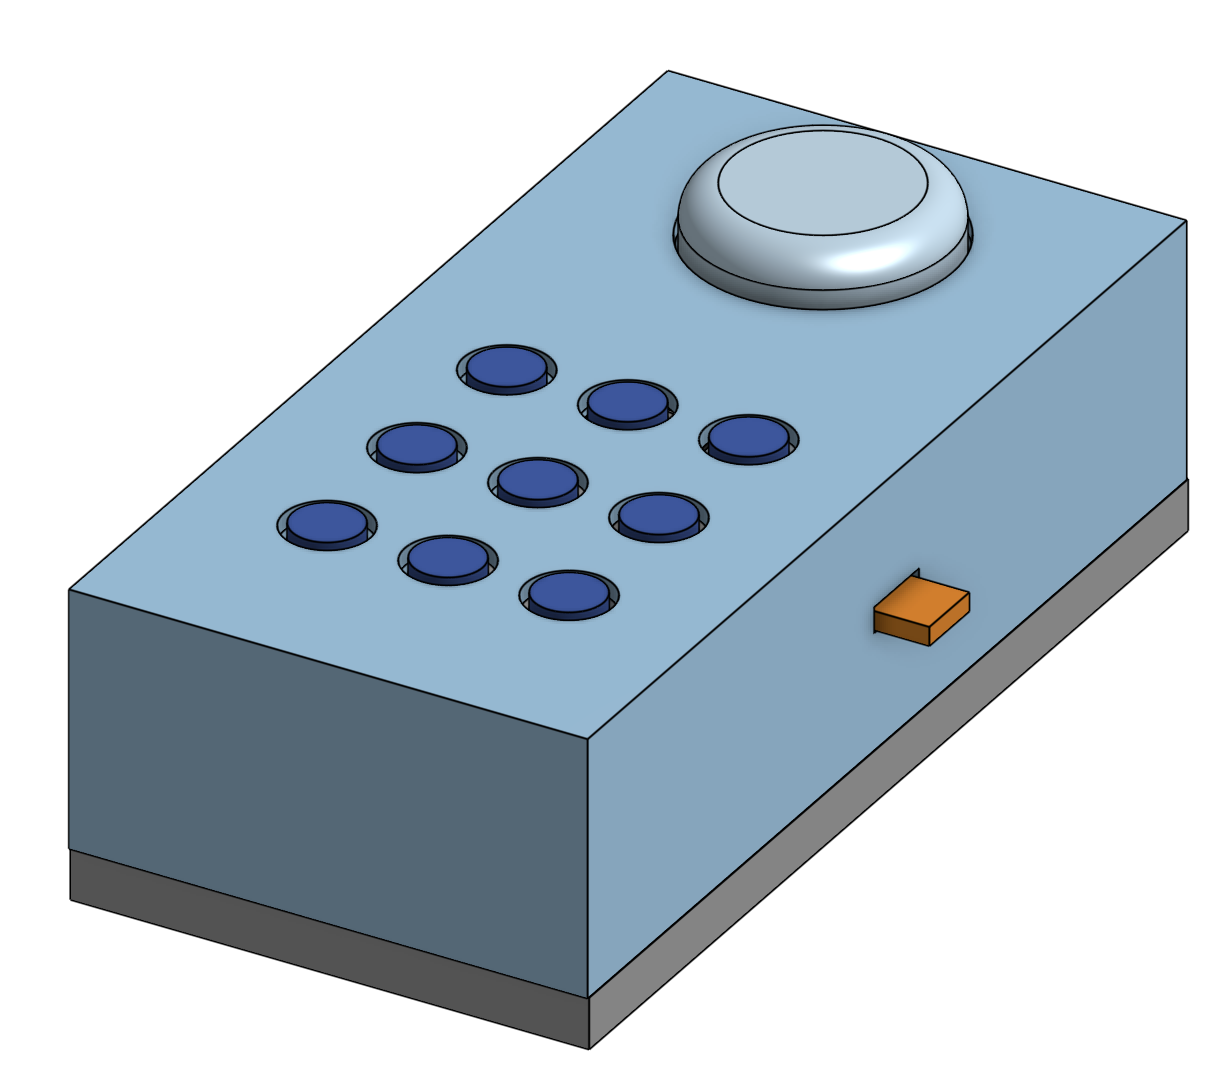
\includegraphics[width=\textwidth]{./isoView.png}
        \caption{Isometric View}
        \label{fig:isoView}
    \end{subfigure}
    \hfill
    \begin{subfigure}[b]{0.48\textwidth}
        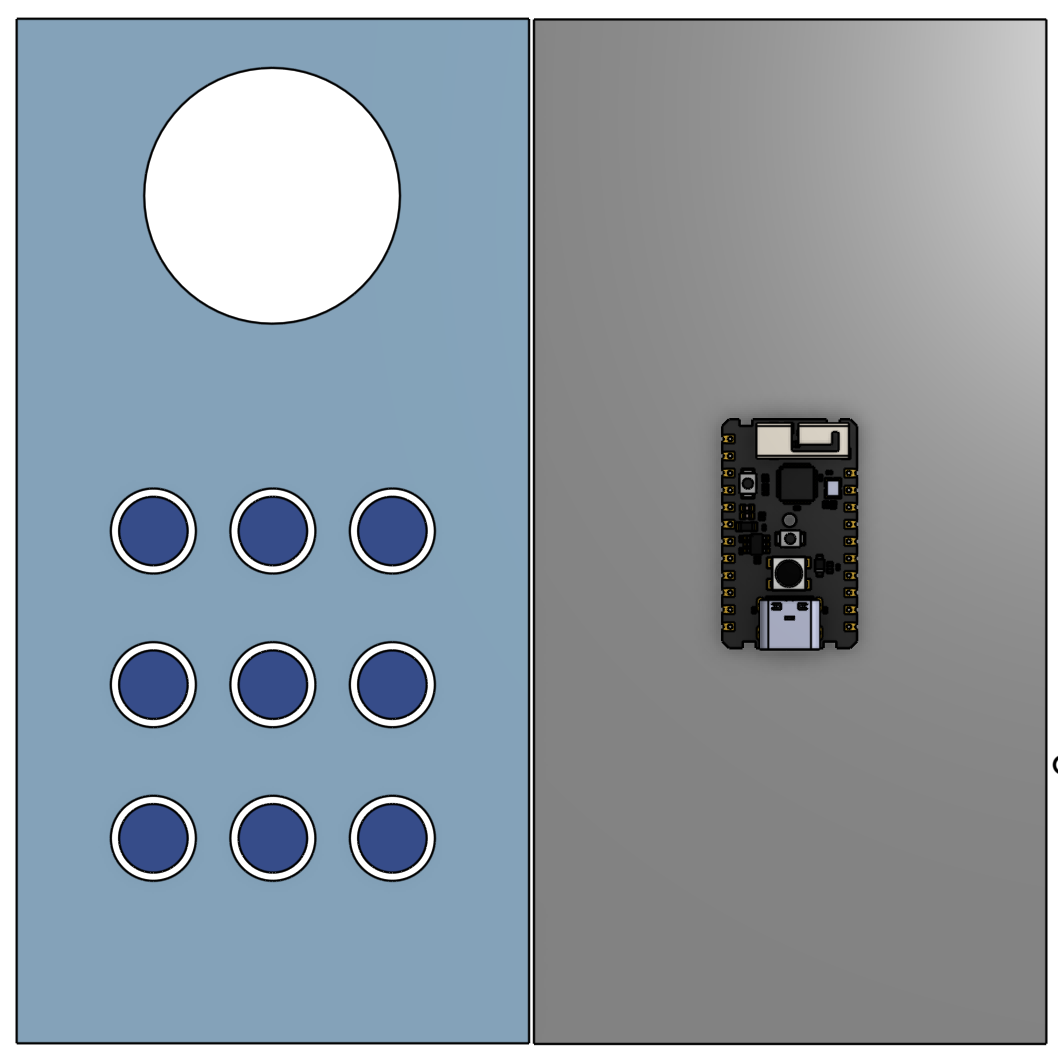
\includegraphics[width=\textwidth]{./topView.png}
        \caption{Top View}
        \label{fig:topView}
    \end{subfigure}
    \caption{First lock design}
\end{figure}

Here is the isometric view of the Smart Lock prototype. The top section will potentially include a biometric scanner, for fingerprint or facial recognition authentication, and a numeric keypad for PIN entry.\newline

\textbf{Key components:}
\begin{itemize}
    \item \textbf{Biometric Scanner:} Supports fingerprint or facial recognition for enhanced security
    \item \textbf{Numeric Keypad:} Users enter PIN codes as an alternative authentication method
    \item \textbf{Solenoid Lock:} Engages or disengages upon successful authentication
    \item \textbf{Microcontroller (ESP32-C3):} Handles user input, authentication, and connectivity
    \item \textbf{Rechargeable Battery:} Powers the system, ensuring reliability even in case of power outages
\end{itemize}

This design ensures compactness while maintaining modular repairability, allowing components to be easily accessed or replaced.


\subsubsection{\textcolor{teal}{Life Cycle Assessment (LCA)}}

The life cycle of the Smart Lock was analyzed to ensure sustainability and environmental responsibility. Key aspects include: \newline

\textbf{Eco-Friendly Manufacturing}
\begin{itemize}
    \item Uses locally sourced materials to minimize transportation emissions
    \item Modular design allows for easy repair and component replacement, reducing e-waste
    \item Prioritizes recyclable materials in construction
\end{itemize}

\textbf{Energy Efficiency}
\begin{itemize}
    \item Operates on a rechargeable lithium battery to extend lifespan
    \item Supports an optional solar charging module to reduce reliance on disposable batteries
\end{itemize}

% Begin Morphological Charts ----------------------------------

\section{Economic Analysis}
Below we have the images for DFM, DFA, and Life Cycle Assessment.
\newpage
\subsection*{DFM \& DFA}
\begin{figure}[!ht]
    \centering
    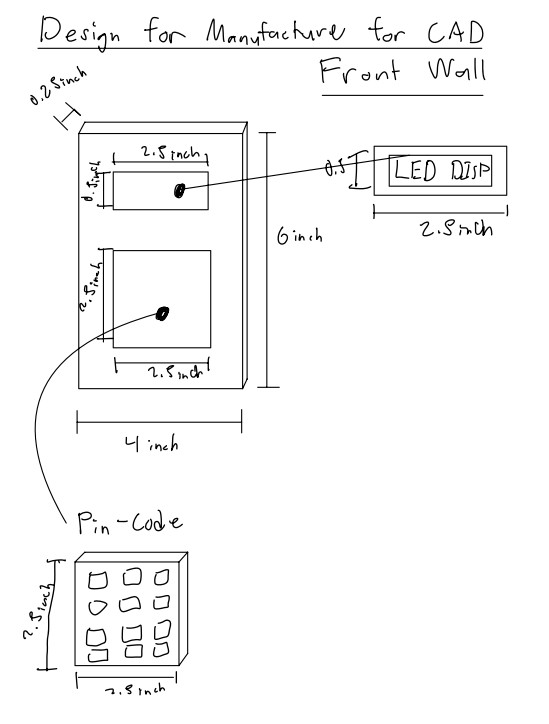
\includegraphics[width=0.8\linewidth]{img/DFM_Front_wall.png}
    % \caption{Physical Solution Chart}
    \label{fig:enter-label}
\end{figure}
\newpage

\begin{figure}[!ht]
    \centering
    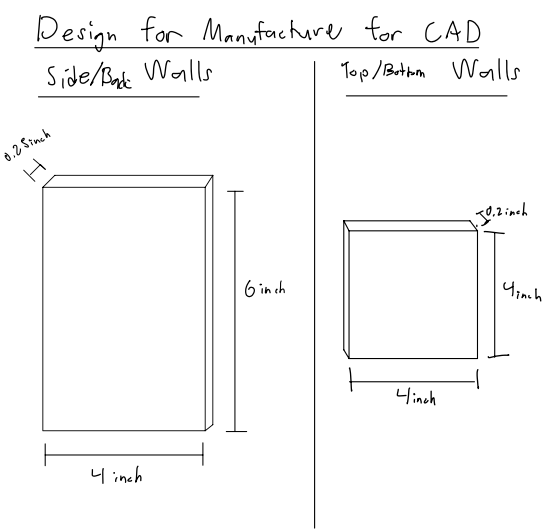
\includegraphics[width=0.8\linewidth]{img/DFM_Side_and_top_wall.png}
    % \caption{Physical Solution Chart}
    \label{fig:enter-label}
\end{figure}
\newpage
\subsection{\textcolor{gray}{Outstanding Issues}}
\textcolor{teal}{\textbf{Hardware/Physical}}
\begin{itemize}
    \item Need to find solenoid lock compatible with ESP32-C3 for testing
    \item Need to make sure generated and customized PINs work with hardware authorization/verification within physical keypad
     \item Need to find battery pack with lifespan of 1.5yrs+
     \item Need to find keypad that can be wired securely to ESP32-C3 in lock 
\end{itemize}
\textcolor{teal}{\textbf{Software/Online}}
\begin{itemize}
     \item Need to print and ensure CAD design works using 123A printers
     \item Programming correct PIN interface storage with secure random generation
     \item 
    
\end{itemize}

\section{Appendices}

\textcolor{teal}{\subsection{Scope}}
\subsubsection*{Firebase Mobile Connectivity Test}
\subparagraph{Test Goals and Purpose}
\begin{itemize}
    \item Ensure that an IOS device can securely connect and push data to the Firebase Firestore servers.
    \item What happens when there may be bad network connection
    \item Set a certain time frame for the pin to be qualified for
\end{itemize}

\subparagraph{Parameters}
\begin{itemize}
    \item 1/0 LOCK$\_$STATE necessary for defining lock-state, 1 is unlocked, 0 is locked.
    \item 7 digit QUALIFIED$\_$PIN list on an allow list for physical keypad on SmartLock.
    \item Make sure what data we send from phone is on firebase
    \item Provide time frame as input for start and expiration time for pin code
\end{itemize}

\subparagraph{Expectations of Test}
\begin{itemize}
    \item There will be no issue with pushing a simple piece of data for LOCK$\_$STATE to the firestore servers, clicking lock will properly push a 0 and clicking unlock will store a 1. Additionally, the pin list composed of generated and custom user pins will also have no trouble being communicated with Firestore servers to later be fetched by the physical device as an additional mechanism for locking and unlocking.
    \item Testing the time frame of the pin code, ensure only the time when valid to use the pin. Otherwise other times should be invalid.
\end{itemize}

\subsubsection{Lock Hardware Functionality Test}
\subparagraph{Test Goals and Purpose}
\begin{itemize}
    \item Ensure that an ESP32-C3 device can securely connect and retrieve data from the Firebase Firestore servers.
    \item Ensure that the ESP32-C3 board can correctly interact with hardware to enable mechanisms for locking/unlocking.
    \item Ensure that invalid codes should not release bolt, while valid codes should.
\end{itemize}


\subparagraph{Parameters}
\begin{itemize}
    \item 1/0 LOCK$\_$STATE necessary for defining lock-state, 0 is locked, 1 is unlocked. Retrieved from firebase.
    \item 7 digit QUALIFIED$\_$PIN list on an allow list for physical keypad on SmartLock.
\end{itemize}

\subparagraph{Expectations of Test}
\begin{itemize}
    \item The locking mechanism will respond appropriately after retrieving from Firestore, and the bolt will trigger when the parameter is set to 0 and likewise release given a 1 value. Additionally, the bolt will release given a valid input from the QUALIFIED$\_$PIN list and reject other non-valid input pins.
    \item Expecting the lock to not unlock after a code is expired, only unlock when it is still valid in a time frame.
\end{itemize}

\subsubsection{Multi-User \& Concurrency Test (Low Priority)}
\subparagraph{Test Goals and Purpose}
\begin{itemize}
    \item Ensure that multiple users can simultaneously interact with the smart lock through the mobile app and keypad without causing system conflicts.
    \item Verify that Firebase can handle concurrent updates to the lock state and PIN list without failure.
    \item Ensure the lock responds appropriately when multiple unlock requests are received from different users.
\end{itemize}


\subparagraph{Parameters}
\begin{itemize}
    \item Simultaneous requests from different mobile devices attempting to unlock/lock the door.
    \item Simultaneous PIN entries from different users on the physical keypad and mobile app.
\end{itemize}

\subparagraph{Expectations of Test}
\begin{itemize}
    \item Multiple users attempting to unlock the door at the same time should not cause conflicts or undefined behavior.
    \item The lock should process and execute the most recent valid request, ensuring no delays or duplicate actions.
    \item System logs should correctly track each user’s request, ensuring accountability and reliable data collection for user feedback.
\end{itemize}
\newpage

% New Section ----------------------------------------------------------------------------------------
\textcolor{teal}{\subsection*{Administrative Details}}

\subsubsection{Firebase Mobile Connectivity Test}
\textbf{\textit{Date $\&$ Location:}} Mar 12, 2025 in class
\newline
\textbf{\textit{Conducting Test:}} Jackson Kennedy, Adam Wu, Nathaniel Laurente, Neena Nguyen, and Professor Harrison.

\subsubsection{Lock Hardware Functionality Test}
\textbf{\textit{Date $\&$ Location:}} Mar 31, 2025 in class
\newline
\textbf{\textit{Conducting Test:}} Jackson Kennedy, Adam Wu, Nathaniel Laurente, Neena Nguyen, and Professor Harrison.

\subsubsection{Multi-User \& Concurrency Test}
\textbf{\textit{Date $\&$ Location:}} April 18, 2025 in class
\newline
\textbf{\textit{Conducting Test:}} Jackson Kennedy, Adam Wu, Nathaniel Laurente, Neena Nguyen, and Professor Harrison.

\textcolor{teal}{\subsection*{Design of Experiment}}
\subsubsection{Firebase Mobile Connectivity Test}
\textbf{\textit{Testing method type:}} Functional Testing, does the simple job of sending unlock or lock to firebase server, also sending pins.
\newline
\textbf{\textit{Test apparatus:}} Firebase Cloud service
\newline
\textbf{\textit{Independent Variables:}} Lock Status, Acceptable Pins
\newline
\textbf{\textit{Dependent Variables:}} N/A
\newline
\textbf{\textit{Number of factors:}}
\newline
\textbf{\textit{Sampling Procedures:}} 2 samples of observing Firestore for 1/0 LOCK$\_$STATE. 2 randomly generated PINs and 1 custom-user pin.

\subsubsection{Lock Hardware Functionality Test}
\textbf{\textit{Testing method type:}} When phone sends data for unlock or lock onto firebase, the lock should quickly retrieve information and respond accordingly. The purpose of this is to make sure the lock receives the data fast enough so that people waiting outside the lock does not wait too long for door to unlock. This should also be similar for the pin code case.
\newline
\textbf{\textit{Test apparatus:}} Utilize ESP32-C3 alongside a Solenoid door lock.
\newline
\textbf{\textit{Independent Variables:}} Make sure that the ESP32-C3 can read a simple "Hello world" on the server for basic testing.
\newline
\textbf{\textit{Dependent Variables:}} Everytime we are generating a new code from phone to firebase, the ESP32-C3 should also be able to retrieve those codes as valid codes immediately.
\newline
\textbf{\textit{Number of factors:}} N/A factors considered in this moment
\newline
\textbf{\textit{Sampling Procedures:}} Samples obtained from servers for LOCK\_STATE, only 0 or 1. Then we have samples for pin codes as well from Firebase.
\newline

\subsubsection{Multi-User \& Concurrency Test}
\textbf{\textit{Testing method type:}} Multiple phones will send an unlock signal from phone at nearly the exact same time and see if any undefined behavior occurs. Send a lock signal and an unlock signal at the same time to test if we can prioritize actions that came first, or lock the app after an action from one device has been made.
\newline
\textbf{\textit{Test apparatus:}} Mobile Device along with ESP32-C3.
\newline
\textbf{\textit{Independent Variables:}} Make sure that the ESP32-C3 can read a simple "Hello world" on the server for basic testing.
\newline
\textbf{\textit{Dependent Variables:}} ESP32-C3 behavior after multiple devices send a signal at the same time or immediately one after the other.
\newline
\textbf{\textit{Number of factors:}} 2 factors to be considered
\newline
\textbf{\textit{Sampling Procedures:}} Samples obtained from servers for LOCK\_STATE, only 0 or 1. Determine if multiple signals causes undefined or expected behavior.



\textcolor{teal}{\subsection*{Testing Procedures}}
\subsubsection{Safety Precautions}
Safety precautions for our project includes not having fast and forceful locks that can hurt individuals.

\subsubsection{Data Collection Method}
Collect data from the phone providing the custom pins onto firebase, as well as collecting data for locking or unlocking. We will also note down which users are grouped together to be able to use the same pin for unlcocking door.

\subsubsection{Observation of External Factors}
Some external factors that could make our product not function properly could include:

\begin{itemize}
    \item Bad network connection from phone or from ESP32-C3
    \item Firebase not loading properly
\end{itemize}

\subsection{Test Results}

\subsubsection{From Test Plan}
We will be testing our Firebase mobile connectivity, Esp32 hardware functionality, and multi-user and concurrency. For each of the tests, I will provide step by step instructions.

In the first test for Firebase mobile connectivity, we will test the connection between the mobile app and the firestore database. We will first build the mobile app and connect the firebase API keys to the app. Then with the mobile app, we will test the connection to the firestore database by sending a value to the database document. We can check if this succeeds by checking the firebase console and seeing if the value is updated.

In the second test for the ESP32 hardware functionality, we will test the connection between the ESP32 and wifi. Once connected to wifi, we will test the connection to the firestore database by using the API keys provided by firebase. Then we will create a document in the firestore database and use the ESP32 to fetch the document data. We can check if this succeeds by checking the fetched data is the same as the data in the firestore database. Also from the hardware functionality test, we are going to test the functionality of the solenoid lock, making sure that we can send a signal to unlock and lock the solenoid lock. One more test that we will need to take into consideration is the keypad functionality. We will test the functionality of the keypad by making sure that we can read the input from the keypad and send the input to the ESP32.

In the third test for multi-user and concurrency, we will test the connection between multiple mobile apps and the firestore database. We will first build the mobile app and connect the firebase API keys to the app. Then with the mobile app, we will test the connection to the firestore database by sending a value to the database document. We can check if this succeeds by checking the firebase console and seeing if the value is updated. We will then test the connection between multiple mobile apps and the firestore database by sending values to the database document from multiple mobile apps. We can check if this succeeds by checking the firebase console and seeing if the values are updated.

% GPT table
\subsubsection{Test Result Summary Table}
\begin{table}[h]
    \centering
    \resizebox{\textwidth}{!}{ % Resizes table to fit within page width
    \rowcolors{2}{teal!10}{teal!25}
    \begin{tabular}{|l|c|c|p{6cm}|}
        \hline
        \rowcolor{teal!50}
        \textbf{Objective ( Target )} & \textbf{Result} & \textbf{Met?} & \textbf{Discussion} \\
        \hline
        Firebase Connectivity & Appropriate 1/0 & N/A & Half this test done - explain how lock/unlock work but haven't tested PINs yet. \\
        
        Lock Hardware Functionality & N/A -\textit{Mar 31, 2025} & N/A & While this test has not been conducted yet, we suspect we will pass this test as the Firebase - Firestore lock/unlock was already successful, and the appropriate data was well-received by the ESP32-C3. All that remains is to ensure that the solenoid lock responds properly to an input signal, as well as compares and responds accordingly to valid/invalid codes. \\
        
        Concurrency & N/A -\textit{April 18, 2025} & N/A & While this test has not been conducted yet, we suspect that we will pass this test. Firebase should be able to handle multiple calls close to each other, as well as transmit this signal in the appropriate order. The Firestore database updated extremely quickly in real-time and shouldn't have trouble with concurrent calls. The PIN entries from different users also shouldn't cause conflict, and the door should unlock/lock as intended. \\
        
        \hline
    \end{tabular}}
\end{table}


\end{document}